\documentclass[14pt]{article}

\usepackage[russian]{babel}
\usepackage{amsmath,amssymb}
\usepackage{parskip}
\usepackage{caption}
\usepackage{textcomp}
\usepackage{gensymb}
\usepackage[dvips]{graphicx}
\usepackage{wrapfig}
\usepackage{color}
\usepackage{setspace}
\usepackage{hyperref}
\usepackage{epstopdf}

\oddsidemargin=0 cm
\evensidemargin=0 cm
\textwidth=170 mm
\textheight=230 mm
\topmargin=0 cm
\voffset= -2cm
\pagenumbering{false}
\newlength{\varheight}
\setlength{\varheight}{3.1cm}
\setlength{\parindent}{0cm}
\spacing{1.1}
\parskip=2mm
\clubpenalty=10000
\widowpenalty=10000

\begin{document}

1. First we evaluate $\vec{d}=\vec{b}\times\vec{c}$:
$$
  \vec{d}=\begin{vmatrix}
  \vec{i} & \vec{j} & \vec{k}\\
  1 & 1 & -1\\
  -1 & 1 & 1
  \end{vmatrix}=2\vec{i}+2\vec{k}.
$$
Then,
\begin{gather}
  \vec{a}\cdot\vec{d}=2-0+2=4,\nonumber\\
  \vec{a}\times\vec{d}=\begin{vmatrix}
  \vec{i} & \vec{j} & \vec{k}\\
  1 & -1 & 1\\
  2 & 0 & 2
  \end{vmatrix}=-2\vec{i}-2\vec{k}.\nonumber
\end{gather}

2. True

3. I don't think a correlation exists (see pic).

\begin{figure}[h]
\begin{center}
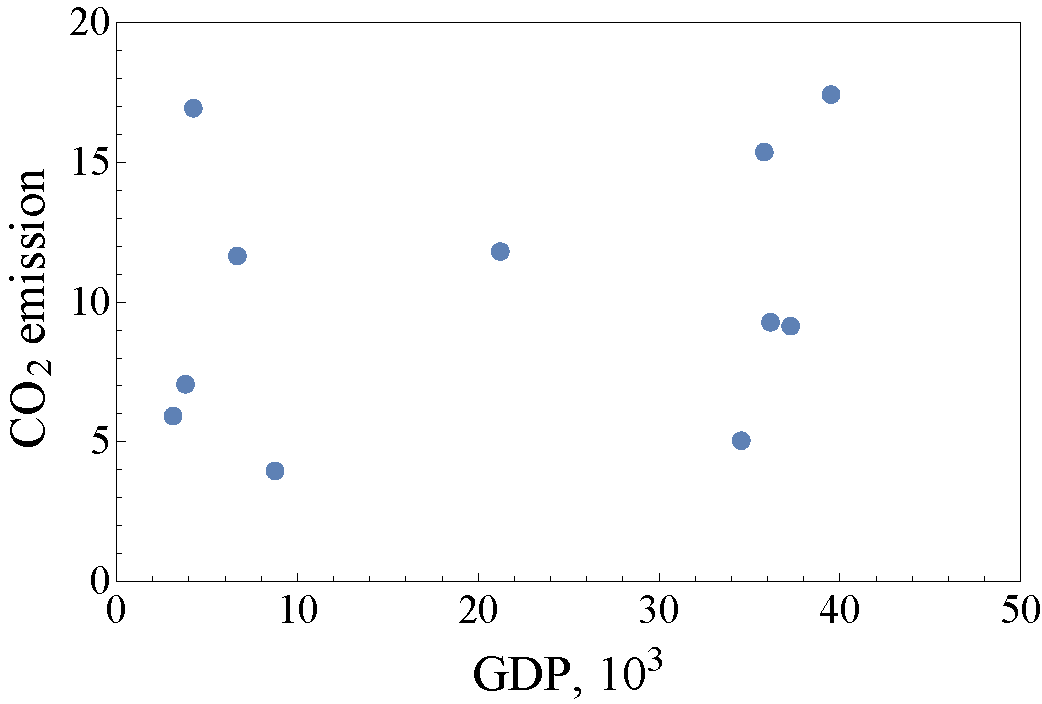
\includegraphics[scale=0.6]{task1pic1.pdf}
\end{center}
\end{figure}

4. The distance $x$ between fringe maxima (or minima) is given by
$$
  x=\frac{\lambda D}{2d}.
$$
Measurements of small fibres may be based on diffraction on a thin wire, for which $x\propto \lambda D/r$, where $r$ is the radius of the wire. The coefficient of proportionality is of order 1 and can be found from geometry.

5. The energy of one photon is
$$
  E_0=\frac{hc}{\lambda}=2.07\text{ eV},
$$
so the work per electron is
$$
  W=E_0-E_\text{max}=0.13\text{ eV}.
$$

6. The capacitor $C_1$ is charged to voltage $V_1=6$ V, so the charge on the top plate is $Q=C_1 V_1=18$ \micro C.

7. The cinema screen should reflect light in all directions as much equally as it can. The mirror only lets a person see a bright spot on the screen, without seeing all the picture.

\end{document} 